\twocolumn[
\begin{center}
\title{\color[cmyk]{1, 0.57, 0, 0.38}{\Huge\bfseries Servizi di sistema (demoni)\\}} % definisco il titolo dell'articolo
\author{\scriptsize Gabriele Trombini (mailga@fedoraonline.it)} % definisco l'autore e altre informazioni
\date{}
\end{center}
{\color[cmyk]{1, 0.46, 0, 0}\LARGE (Parte prima) I servizi in Fedora - introduzione}\\
\maketitle
\normalsize
\doublespacing
\hfill
]
\definecolor{shadecolor}{cmyk}{0, 0, 0, 0.8}
\onehalfspacing
\lettrine[lines=1, loversize=0.1, lraise=0.1]{\color[cmyk]{0.5, 0, 1, 0}\bfseries C}{}ominciamo a dare una occhiata al sistema di gestione dei servizi che recentemente ha cominciato a sostituire {\itshape SysVinit} ed {\itshape Upstart} nell'avvio e nella gestione dei servizi.\\

I collaboratori italiani del team di traduttori del Fedora Project hanno preparato la pagina wiki {\itshape https://fedoraproject.org/ wiki/Features/systemd/it} dove sono ben spiegati i vantaggi di questo sistema di gestione della sessione e del sistema.\\

\begin{figure*}[!htbp]
\centering
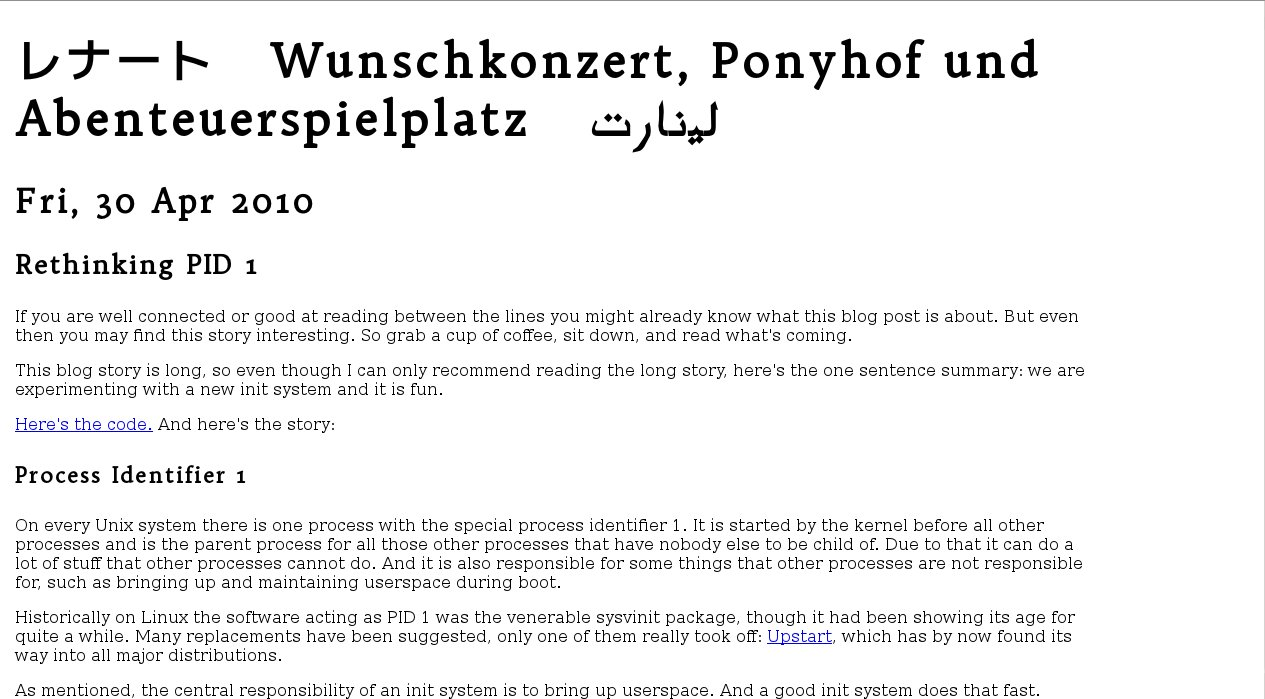
\includegraphics[scale=.45]{articoli/sistema_base/immagini/home_systemd.jpeg}
\caption{pagina del progetto ({\scriptsize http://0pointer.de/blog/projects/systemd.html})}
\end{figure*}

Facendo riferimento alla pagina del wiki\\{\itshape http://fedoraproject.org/wiki/Systemd},\\ dove troviamo dettagliatamente descritte le funzionalità, tra gli altri vantaggi notiamo che {\itshape systemd} velocizza l'avvio attivando processi in parallelo dando l'ascolto ai sockets prima di assegnare loro il servizio.\\

Il sistema {\itshape init} provvedeva a creare prima tutti i sockets e poi tutti i servizi, creando, in caso di dipendenza di un servizio rispetto ad un altro non ancora avviato, l'eventuale stallo del sistema o il mancato avvio del servizio stesso.\\

Inoltre esso si appoggia a D-Bus per l'avvio dei servizi on-demand, permette un recupero del sistema in caso di problemi (previo snapshot), si occupa del mount e dell'automount dei device (fstab può essere utilizzato come configurazione extra, indicando a {\itshape systemd} di monitorarlo), mantiene compatibilità con i sistemi precedenti e può essere configurato, praticamente, a piacimento.\\

Perciò, di fatto, a partire da Fedora 16 la nostra distribuzione ha introdotto in maniera massiva {\itshape systemd} per l'avvio e la gestione dei servizi.\\

Quali sono i vantaggi li abbiamo visti, seppur sommariamente (per approfondimenti dovremo studiarci le pagine web citate in precedenza), ma quello che più ci preme è la loro gestione.\\

Per facilitare il compito possiamo installare {\itshape systemadm} che ci fornisce una GUI con dei comandi minimali per l'avvio/ar\-resto/riavvio dei servizi, per esaminarli e per effettuare lo snapshot di cui sopra:

\begin{shaded}
{\color[cmyk]{0, 0, 0, 0}\#\ yum install systemd-gtk}
\end{shaded}
e per avviarlo: 
\begin{shaded}
{\color[cmyk]{0, 0, 0, 0}\textdollar\ systemadm}
\end{shaded}

Inutile dire che utilizzando il terminale possiamo fruire dei vantaggi della velocità di esecuzione uniti alle opzioni dei comandi.\\

Il tool testuale è {\itshape systemctl}, il cui utilizzo completo può essere studiato nelle pagine man:

\begin{shaded}
{\color[cmyk]{0, 0, 0, 0}\textdollar\ man systemctl}
\end{shaded}

\begin{figure*}[!htbp]
\centering
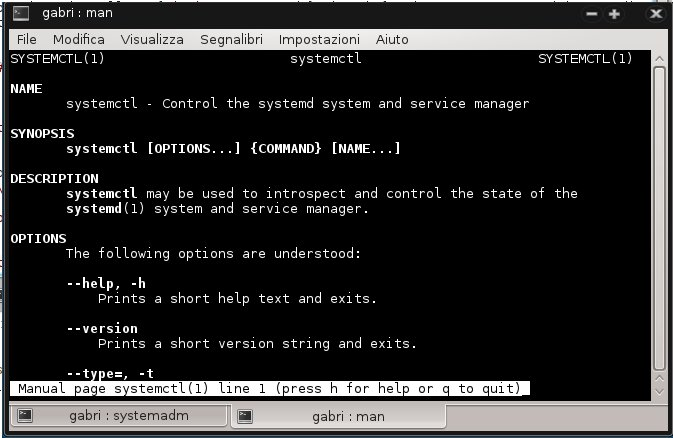
\includegraphics[scale=.80]{articoli/sistema_base/immagini/man_systemctl.jpeg}
\caption{pagina del manuale di systemctl}
\end{figure*}

Questo comando permette di effettuare tutte le principali operazioni di cui un utente potrebbe avere bisogno e la sintassi è molto semplice e, in qualche caso, ricorda l'utilizzo del comando ``service'', con il quale mantiene una certa compatibilità prima di essere totalmente abbandonato in futuro.
\begin{itemize}
\item verificare i servizi
\begin{shaded}
{\color[cmyk]{0, 0, 0, 0}\textdollar\ systemctl list-units --type=service}
\end{shaded}
\item verificare lo stato di un servizio
\begin{shaded}
{\color[cmyk]{0, 0, 0, 0}\textdollar\ systemctl status nome.service}
\end{shaded}
\item informazioni approfondite sullo stato di un servizio attivo
\begin{shaded}
{\color[cmyk]{0, 0, 0, 0}\textdollar\ systemctl is-active nome.service}
\end{shaded}
\item abilitare un servizio all'avvio
\begin{shaded}
{\color[cmyk]{0, 0, 0, 0}\#\ systemctl enable nome.service}
\end{shaded}
\item disabilitare un servizio all'avvio
\begin{shaded}
{\color[cmyk]{0, 0, 0, 0}\#\ systemctl disable nome.service}
\end{shaded}
\item avviare un servizio
\begin{shaded}
{\color[cmyk]{0, 0, 0, 0}\#\ systemctl start nome.service}
\end{shaded}
\item fermare un servizio
\begin{shaded}
{\color[cmyk]{0, 0, 0, 0}\#\ systemctl stop nome.service}
\end{shaded}
\item riavviare un servizio
\begin{shaded}
{\color[cmyk]{0, 0, 0, 0}\#\ systemctl restart nome.service}
\end{shaded}
\item ``uccidere'' un servizio
\begin{shaded}
{\color[cmyk]{0, 0, 0, 0}\#\ systemctl kill nome.service}
\end{shaded}
\end{itemize}

Cercando di andare un po' in profondità, possiamo vedere che le directory di riferimento di {\itshape systemd} sono fondamentalmente due:
\begin{itemize}
\item /etc/systemd
\item /lib/systemd 
\end{itemize}

Il contenuto della directory {\itshape /etc/systemd} ha la precedenza tra i due, ma entrambi contengono i servizi disponibili.\\

Ecco il file di configuraizone di mysqld:
\begin{shaded}
{\color[cmyk]{0, 0, 0, 0}[Unit]\\
Description=MySQL database server\\
After=syslog.target\\
After=network.target\\

[Service]\\
Type=forking\\
User=mysql\\
Group=mysql\\

ExecStartPre=/usr/libexec/mysqld-prepare-db-dir\\
\# Note: we set --basedir to prevent probes that might trigger SELinux alarms,\\
\# per bug \#547485\\
ExecStart=/usr/bin/mysqld\_safe --nowatch --basedir=/usr\\
ExecStartPost=/usr/libexec/mysqld-wait-ready \textdollar MAINPID\\

\# Give a reasonable amount of time for the server to start up/shut down\\
TimeoutSec=300\\

\# We rely on systemd, not mysqld\_safe, to restart mysqld if it dies\\
Restart=always\\
{\color[cmyk]{0, 0, 0, 0}[Unit]
[Install]\\
WantedBy=multi-user.target\\
}
}
\end{shaded}

Qualora volessimo creare un servizio, il file di configurazione deve essere inserito all'interno di {\itshape /lib/systemd}, e poi collegato in {\itshape /etc/systemd} così che alla variazione del primo, corrisponda la variazione del secondo.\\

 Per fare in modo che systemd venga a conoscenza del nuovo file:
\begin{shaded}
{\color[cmyk]{0, 0, 0, 0}\#\ systemctl systemctl daemon-reload}
\end{shaded}

Per abilitarlo all'avvio, basta quindi usare l'opzione --enable di cui abbiamo già parlato.\\

L'argomento merita un approfondimento maggiore (e per taluni aspetti ancora da scoprire) rispetto a quanto è possibile fare in un unico numero, tuttavia per un primo approccio al nuovo sistema di gestione dei servizi questo articolo può essere sufficiente.\\

Systemd verrà probabilmente ripreso nei prossimi numeri ad un livello di dettaglio più analitico, con esempi e con la chiamata in causa di {\itshape D-Bus}.\\


\hfill {\itshape (fine prima parte)}




